\documentclass[journal]{IEEEtran}

\usepackage{amsmath,amssymb,amsfonts}
\usepackage{algorithm}
\usepackage{algorithmic}
\usepackage{array}
\usepackage{booktabs}
\usepackage{cite}
\usepackage{graphicx}
\usepackage{multirow}
\usepackage{tikz}
\usepackage{url}
\usepackage{xcolor}
\usetikzlibrary{arrows,positioning,fit,shapes.geometric,calc}

\newcommand{\KG}{\mathcal{G}}
\newcommand{\SG}{\mathcal{S}}
\newcommand{\calA}{\mathcal{A}}
\newcommand{\calC}{\mathcal{C}}
\newcommand{\calD}{\mathcal{D}}
\newcommand{\calE}{\mathcal{E}}
\newcommand{\calI}{\mathcal{I}}
\newcommand{\calN}{\mathcal{N}}
\newcommand{\calQ}{\mathcal{Q}}
\newcommand{\calR}{\mathcal{R}}
\newcommand{\calS}{\mathcal{S}}
\newcommand{\calV}{\mathcal{V}}
\newcommand{\bbE}{\mathbb{E}}
\newcommand{\R}{\mathbb{R}}
\newcommand{\one}{\mathbf{1}}

\begin{document}

\title{Intent-Conditioned Knowledge-Graph Pruning and Imitation Reasoning for LLM-Free Semantic Communications}

\author{Xinyu~Xie%
\thanks{X. Xie is with the Chongqing University of Posts and Telecommunications, Chongqing 400065, China (e-mail: s250131112@stu.cqupt.edu.cn).}}

\markboth{}{}

\maketitle

\begin{abstract}
Semantic communication aims to deliver task-relevant meaning rather than bit-exact replicas. Recent implicit semantic-aware designs show that a receiver can recover hidden relations and entities by reasoning over background knowledge; however, many emerging intent-driven schemes rely on large language models, large action models, or remote generative services for semantic extraction and policy adaptation. Such dependence can be undesirable in latency-critical, privacy-sensitive, or reproducibility-oriented wireless systems. This paper develops an LLM-free knowledge-graph (KG) semantic communication framework in which the source intent is converted into a compact dynamic subgraph through deterministic keyword extraction, TransE-space semantic matching, out-of-distribution (OOD) entity injection, and bounded breadth-first-search (BFS) pruning. The destination interprets the selected semantics with a graph convolutional network (GCN) and a generative-adversarial imitation learning (GAIL) policy over a Semi-Markov decision process (Semi-MDP). A fixed 452-dimensional state contract concatenates the current-node representation, subgraph representation, intent embedding, and channel-state information (CSI), thereby separating slow semantic graph updates from fast wireless control. We formulate the source-destination-common-KB system model, derive an intent-conditioned pruning objective, present the offline training and online communication algorithms, and analyze pruning radius, OOD stability, and spectral-normalized policy jumps. Prototype traces on FB15K237-style KG experiments indicate that the dual-loop architecture reduces online semantic-control latency from about 1.2 s to a few milliseconds while preserving interpretable KG paths. The resulting framework provides a reproducible TWC-style baseline for implicit semantic-aware communication without LLM/LAM APIs.
\end{abstract}

\begin{IEEEkeywords}
Semantic communication, implicit semantics, knowledge graph, intent-driven networking, TransE, GAIL, Semi-MDP, graph neural networks, OOD injection.
\end{IEEEkeywords}

\section{Introduction}

Classical communication theory studies how to reproduce symbols reliably over a noisy channel \cite{shannon1948mathematical}. Its separation principle, coding theorems, and information measures remain foundational for wireless systems. Nevertheless, many future services do not need every transmitted bit to be recovered exactly. A vehicle needs the meaning of a warning before the warning becomes obsolete; a robot needs the next task-relevant relation in a scene graph; a remote medical controller needs the semantic state that changes a decision \cite{peng2026simac,krayani2026aav,wheeler2025causal}. Semantic communication therefore changes the objective from symbol reproduction to meaning transfer and task satisfaction \cite{shannonweaver1949,nguyen2025survey,zhang2020semantics}.

The recent literature has advanced semantic communication along several directions. Deep joint source-channel coding (JSCC) learns compact continuous representations that degrade gracefully under noisy channels \cite{bourtsoulatze2019deep,yang2022ofdm,gunduz2025jscc,kurka2020feedback,yang2025swinjscc}. Semantic-aware networking connects high-level intent with radio and computing decisions, increasingly with the help of edge AI agents \cite{qin2025genai,sun2026edge,jiang2026agentic}. Knowledge-base-assisted and generative semantic communication systems exploit external background knowledge to recover content that is not explicit in the source signal \cite{xiao2024reasoning,fang2026cross,peng2026simac}. These developments are important because practical human and machine messages contain both explicit semantics, which can be directly recognized from the signal, and implicit semantics, which must be inferred from context, prior knowledge, user background, and task goals.

The work ``Reasoning over the Air'' is particularly relevant to this paper because it frames semantic communication as a reasoning problem over explicit and implicit semantic paths \cite{xiao2024reasoning}. Subsequent imitation-based and structure-aware extensions further develop multi-layer semantic representation, collaborative reasoning, and implicit-semantic recovery \cite{xiao2023imitation,liao2026hypergraph}. In that architecture, the source and destination exploit semantic knowledge bases, and the destination learns an interpreter by imitation-style reasoning. This paper follows the same high-level spirit: a communication system should not merely transmit isolated labels, but should transmit enough structured knowledge for a receiver to infer hidden semantic relations. We depart from that line of work in two practical aspects. First, our implementation is intentionally LLM-free and LAM-free. Intent extraction is implemented by a deterministic keyword table, not by a remote language model. Second, the semantic reasoning substrate is a dynamically pruned KG subgraph whose size is bounded before the fast wireless control loop executes. This makes the system easier to audit, easier to reproduce, and more suitable for latency-sensitive experiments.

The motivating observation is simple. A large KG is valuable because it provides typed entities and relations, but it is too large to expose directly to a fast wireless controller. Conversely, a small static subgraph is efficient, but it cannot adapt to user intent or unknown entities. We therefore split the system into a slow semantic loop and a fast decision loop. The slow loop resolves intent keywords into KG seeds, injects OOD entities if the intent cannot be reliably matched, and prunes a bounded subgraph. The fast loop treats that subgraph as a local semantic state space and repeatedly chooses KG-path and radio-control actions. The central engineering invariant is
\begin{equation}
\label{eq:state_contract_intro}
d_s = 256 + 128 + 64 + 4 = 452,
\end{equation}
where the four terms are the current-node embedding, GCN subgraph embedding, intent embedding, and compact CSI vector. This 452-dimensional contract is enforced in the code base and is treated as a non-negotiable interface between semantic processing and control learning.

This design addresses three difficulties that repeatedly appear in semantic communication prototypes. The first is semantic selection: only a small subset of a KG is relevant to a given intent, and the selection must be done before channel-control decisions are made. The second is semantic novelty: a user may mention an entity that is not present in the initial KG, and dropping it destroys the very semantics that the system should preserve. The third is non-stationarity: the relevant KG region changes when the user intent changes, so the policy must remain stable under subgraph replacement. Our solution combines TransE-space matching, nearest-neighbor OOD injection, bounded BFS, GCN encoding, and spectral-normalized GAIL to address these issues in a single reproducible pipeline \cite{bordes2013translating,kipf2017semi,ho2016gail,miyato2018spectral}.

The contributions of this paper are summarized as follows.
\begin{itemize}
\item We formulate an LLM-free implicit semantic-aware communication model with source-user KG, destination-user KG, a shared common KG, and a noisy wireless channel. The model follows the Transactions-style semantic reasoning view while using a deterministic, locally reproducible intent interface \cite{xiao2024reasoning,fang2026cross,liao2026hypergraph}.
\item We develop an intent-conditioned dynamic KG pruning method that maps keywords to TransE-space seed entities, injects unmatched OOD entities into the KG, and extracts a bounded BFS subgraph with at most 64 nodes \cite{xie2016transe,bordes2013translating}.
\item We cast fast semantic interpretation and resource-aware KG navigation as a Semi-MDP and solve it with a GAIL-style policy and discriminator \cite{puterman1994mdp,ho2016gail,zhang2025heteroknowledge}. The policy consumes a fixed 452-dimensional state and is therefore decoupled from changes in the slow semantic loop.
\item We derive practical criteria for pruning radius, OOD perturbation stability, intent-switching policy jumps, and amortized latency. These results explain why bounded subgraphs and spectral normalization are useful rather than merely convenient \cite{miyato2018spectral,kipf2017semi}.
\item We provide a prototype evaluation pipeline over FB15K237/WN18RR/NELL-style KG settings \cite{toutanova2015observed,dettmers2018conve}, including convergence traces, latency decomposition, OOD robustness, threshold ablation, BFS/GCN profiling, and TransE semantic-decay measurements.
\end{itemize}

The rest of this paper is organized as follows. Section~II reviews related work. Section~III presents the system model. Section~IV formulates the optimization problem. Section~V describes the proposed dynamic KG pruning and imitation reasoning method. Section~VI gives the algorithms and complexity analysis. Section~VII presents analytical properties. Section~VIII reports prototype evaluations. Section~IX details protocol operation and synchronization, and Section~X concludes the paper.

\section{Related Work}

\subsection{Semantic Communication}

Semantic communication can be traced to the distinction between technical, semantic, and effectiveness levels of communication \cite{shannonweaver1949}. Modern work operationalizes this idea by learning representations that are sufficient for downstream tasks, by transmitting semantic symbols, or by using knowledge bases to interpret messages \cite{nguyen2025survey,zhang2020semantics,fang2026cross}. Deep JSCC is one of the most mature branches. It learns an end-to-end source-channel mapping and often outperforms separated compression and channel coding at low signal-to-noise ratios (SNRs) \cite{bourtsoulatze2019deep}. OFDM-guided JSCC further incorporates wireless channel structure into the neural transceiver \cite{yang2022ofdm}, while transformer-based and fidelity-adjustable designs improve adaptivity and edge inference efficiency \cite{yang2025swinjscc,devoto2026token,li2023fast}. These works mostly focus on signal-domain representations such as image, text, or feature tensors. They are complementary to our KG-level method, which performs semantic selection before waveform or bit-level coding \cite{gunduz2025jscc,kurka2020feedback,bourtsoulatze2019deep}.

Implicit semantic-aware communication emphasizes hidden relations, user background, and reasoning paths. A semantic receiver may need to infer that an observed entity implies a hidden relation, or that two possible meanings of the same explicit term should be resolved differently under different user histories. Xiao \emph{et al.} propose a reasoning-based implicit semantic-aware communication framework and a generative adversarial imitation solution for semantic path generation \cite{xiao2024reasoning}. Related efforts pursue implicit semantics through multi-layer imitation reasoning, hypergraph information bottlenecks, and conceptual or causal learning \cite{xiao2023imitation,liao2026hypergraph,wheeler2025causal}. Our work inherits the idea that semantic interpretation can be represented as reasoning over paths, but we replace broad semantic extraction with an auditable KG pruning process and a fixed-dimensional policy interface.

\subsection{Intent-Driven Wireless Systems}

Intent-driven networking maps high-level service objectives into concrete network configurations. Recent work explores generative AI and interactive agents to translate natural-language intent into wireless control actions \cite{qin2025genai}. Related directions include edge large-AI-model agents for cognitive multimodal semantic communication \cite{sun2026edge}, agentic-AI communication tutorials \cite{jiang2026agentic}, and semantic-aware resource allocation driven by Bayesian active inference \cite{krayani2026aav}. Such methods can be powerful because they exploit large-scale pretraining and open-domain language understanding. However, deployment in safety-critical control loops raises concerns about latency, privacy, external API dependence, reproducibility, and verification. Our design deliberately removes LLM/LAM calls. This restriction reduces open-domain expressiveness, but it clarifies what can be achieved with a local KG, deterministic extraction, and imitation control alone.

The LLM-free choice also changes the engineering target. Instead of asking a model to interpret arbitrary text, the system assumes a bounded intent vocabulary aligned with application domains such as collision avoidance, drone surveillance, robot navigation, telemedicine, and smart-grid monitoring. The intent extractor returns a small set of entities, and the KG operations handle the remaining semantic grounding. This separation is useful when the semantic communication stack must be certified, tested offline, or deployed on constrained hardware \cite{jiang2026agentic,sun2026edge,devoto2026token}.

\subsection{Knowledge Graphs and Embedding Models}

KGs encode facts as triples $(h,r,t)$, where $h$ and $t$ are entities and $r$ is a relation. Translation-based KG embeddings such as TransE learn vectors satisfying $\mathbf{z}_h+\mathbf{z}_r\approx \mathbf{z}_t$ for plausible triples \cite{bordes2013translating}. Entity-description-enhanced variants further enrich these representations with auxiliary text \cite{xie2016transe}. FB15K237 and WN18RR are standard benchmarks for KG completion and reasoning \cite{toutanova2015observed,dettmers2018conve}. In this paper, TransE embeddings serve two purposes: they provide node features for subgraph encoding, and they provide a semantic space for intent-keyword matching.

Graph neural networks aggregate neighborhood information and can compress a variable-size graph into a fixed-size representation \cite{kipf2017semi}. The proposed method uses a two-layer GCN with global mean pooling. This is intentionally modest: the paper focuses on the communication architecture and state contract, not on maximizing graph representation performance with a large graph transformer. More expressive graph encoders could be substituted as long as they preserve the subgraph embedding dimension \cite{kipf2017semi,liao2026hypergraph}.

\subsection{Imitation Learning and Semantic Reasoning}

Imitation learning is attractive when reward design is difficult but expert behavior is available. GAIL matches the occupancy measure of an expert policy through an adversarial discriminator \cite{ho2016gail}. Adversarial reinforcement learning has also been used to optimize semantic communication under heterogeneous knowledge \cite{zhang2025heteroknowledge}, and imitation-based reasoning has been applied directly to implicit semantic-aware networks \cite{xiao2023imitation}. In semantic reasoning, expert paths may be generated by a user history, a rule base, a shortest-path oracle, or a domain-specific heuristic. The current implementation uses a BFS-based mock expert so that the training pipeline remains independent of external teachers. This is analogous in spirit to G-RML-style semantic path learning \cite{xiao2024reasoning}, but the expert is generated inside the pruned KG and the learned policy is constrained by the fixed 452-dimensional state.

\section{System Model}

\subsection{Network and Knowledge Architecture}

We consider a source user and a destination user communicating over a wireless channel. Each side has access to a local user-specific KG and a shared common KG. The source observes a message, sensor report, or application event, extracts explicit intent terms, and selects a compact semantic representation for transmission. The destination receives the semantic representation through a noisy channel and reconstructs implicit semantic paths using its interpreter and the available KG context.

Let the common KG be
\begin{equation}
\KG_c=(\calV_c,\calR_c,\calE_c), \quad
\calE_c\subseteq \calV_c\times \calR_c\times \calV_c .
\end{equation}
The source and destination maintain local KGs $\KG_s$ and $\KG_d$, respectively. Their working graph at a communication episode is
\begin{equation}
\KG = \KG_c \cup \KG_s \cup \KG_d \cup \KG_{\mathrm{dyn}},
\end{equation}
where $\KG_{\mathrm{dyn}}$ contains injected OOD entities and dynamic relations discovered by the slow loop. In implementation, the global graph is represented by a directed graph loaded from benchmark triples, and injected nodes receive negative IDs so that they do not collide with benchmark entity IDs.

\begin{figure*}[!t]
\centering
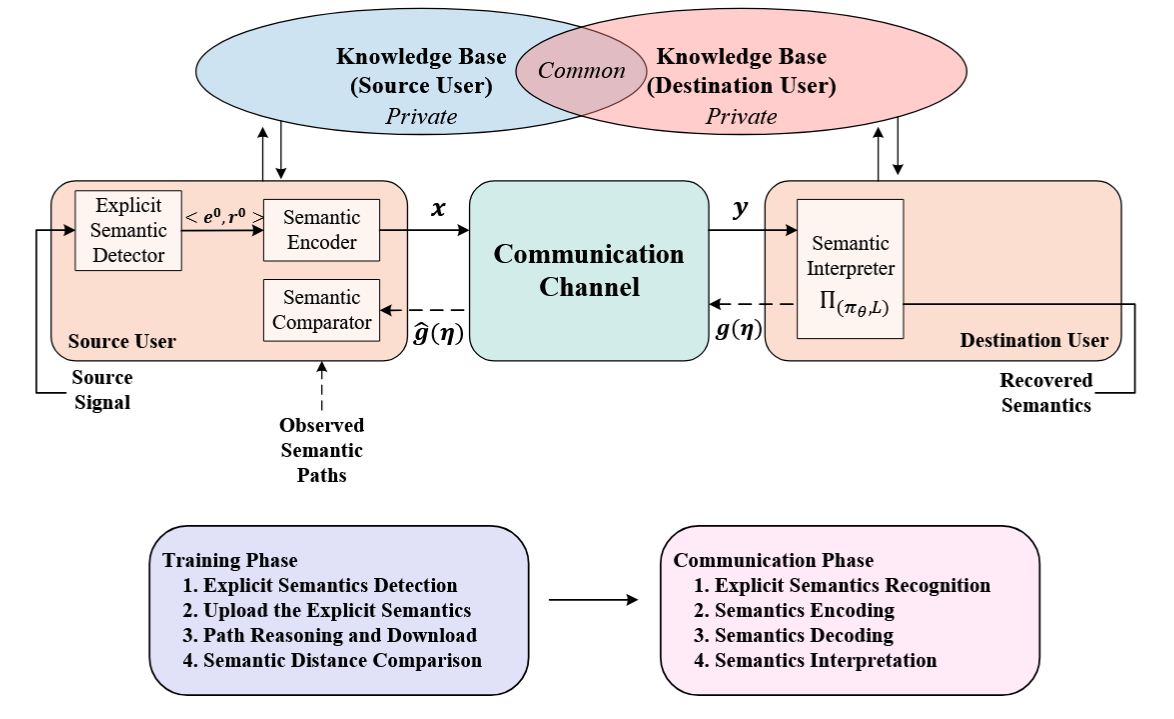
\includegraphics[width=\textwidth]{fig_system_model.png}
\caption{System model for LLM-free implicit semantic-aware communication. The source user and destination user maintain local knowledge bases and share a common KG. During training, the destination learns a semantic interpreter from source-side semantic-distance feedback. During communication, the source transmits compact explicit semantics through the channel and the destination infers intent-conditioned implicit semantic paths.}
\label{fig:system_model}
\end{figure*}

Fig.~\ref{fig:system_model} shows the system model. The layout follows the source-destination semantic reasoning structure commonly used in implicit semantic-aware communication: a training phase aligns the destination interpreter with source-side semantic distance, while a communication phase transmits compact semantics and lets the destination infer hidden meaning locally. Our implementation instantiates the source-side semantic encoder with TransE matching, OOD injection, and BFS pruning, and instantiates the destination interpreter with GCN and GAIL.

\subsection{Explicit and Implicit Semantics}

For a source observation $x$, the explicit semantics are represented as
\begin{equation}
u_0(x)=\langle \calC(x),\calR_0(x)\rangle ,
\end{equation}
where $\calC(x)$ is a set of recognized intent entities and $\calR_0(x)$ is a set of directly observed relations when available. In the current code, $\calC(x)$ is produced by deterministic keyword matching. For example, the keyword ``collision'' maps to entities such as vehicle, collision, brake, and emergency; the keyword ``drone'' maps to drone, surveillance, camera, and video.

Implicit semantics are represented as a path or sequence of hidden entities and relations \cite{sun2026hierarchy,xiao2024reasoning},
\begin{equation}
u_v = \langle (e_1,r_1),(e_2,r_2),\ldots,(e_L,r_L)\rangle,
\end{equation}
where the hidden terms are not necessarily observable from the source signal but are needed for the destination to interpret the meaning. The reasoning policy $\Pi$ maps the explicit semantics, local context, and CSI-aware state to a distribution over next semantic actions:
\begin{equation}
\Pi: (\SG_N,u_0,\mathbf{c}_t,v_t)\mapsto p(a_t|s_t).
\end{equation}
The objective is not to transmit the entire implicit path. Instead, the source selects a compact intent-conditioned subgraph and the destination locally generates the likely path.

\subsection{Wireless Channel and Semantic Symbols}

The physical channel is summarized by a compact CSI vector
\begin{equation}
\mathbf{c}_t =
[\gamma_t/50,\; f_{D,t}/100,\; \widehat{\mathrm{SINR}}_t,\; \widehat{\ell}_t]^\top
\in\R^4,
\label{eq:csi_vector}
\end{equation}
where $\gamma_t$ is sampled SNR in dB, $f_{D,t}$ is Doppler frequency, $\widehat{\mathrm{SINR}}_t$ is normalized SINR, and $\widehat{\ell}_t$ is normalized path loss. The channel can be AWGN or simplified Rayleigh fading:
\begin{equation}
\mathbf{y}_t=h_t\mathbf{x}_t+\mathbf{n}_t,
\end{equation}
where $h_t$ denotes fading and $\mathbf{n}_t$ is additive Gaussian noise \cite{shannon1948mathematical,bourtsoulatze2019deep}. The current prototype does not optimize a complete waveform. Instead, it uses the channel as a stochastic component of the semantic decision state. This is a common first step for KG semantic communication because semantic pruning and reasoning can be evaluated independently before integrating a full PHY encoder.

\subsection{State Contract}

The fast-loop state is
\begin{equation}
\label{eq:state}
\mathbf{s}_t =
\left[\mathbf{z}_{v_t};\mathbf{g}_{\SG};\mathbf{i};\mathbf{c}_t\right]\in\R^{452},
\end{equation}
where $\mathbf{z}_{v_t}\in\R^{256}$ is the current-node embedding consumed by the policy, $\mathbf{g}_{\SG}\in\R^{128}$ is the GCN subgraph embedding, $\mathbf{i}\in\R^{64}$ is the intent vector, and $\mathbf{c}_t\in\R^4$ is the CSI vector in \eqref{eq:csi_vector}. The implementation treats \eqref{eq:state} as a strict contract. If the slow loop changes the number of extracted nodes, injects new OOD entities, or switches intent, the fast loop still receives a state vector of dimension 452.

\begin{table}[!t]
\centering
\caption{State contract and main implementation settings.}
\label{tab:contract}
\begin{tabular}{lcc}
\toprule
Component & Symbol & Dimension / value\\
\midrule
Current-node policy feature & $\mathbf{z}_{v_t}$ & 256\\
GCN subgraph feature & $\mathbf{g}_{\SG}$ & 128\\
Intent feature & $\mathbf{i}$ & 64\\
CSI feature & $\mathbf{c}_t$ & 4\\
\midrule
Policy state & $\mathbf{s}_t$ & 452\\
Discrete action space & $\calA$ & 128\\
Action embedding in discriminator & -- & 8\\
Max pruned subgraph nodes & $|\calV_N|$ & 64\\
TransE/entity matching dimension & -- & 128\\
GCN hidden dimension & -- & 256\\
Policy/discriminator hidden width & -- & 512\\
\bottomrule
\end{tabular}
\end{table}

\section{Problem Formulation}

\subsection{Intent-Conditioned Semantic Selection}

Given an observation $x$ and intent entity set $\calC(x)$, the source must select a subgraph $\SG_N(x)\subseteq \KG$ that preserves the semantic information needed by the destination while satisfying a latency and size budget. Let $\Phi(\SG_N,u_v)$ denote the semantic fidelity between a subgraph and the desired implicit path, and let $T_{\mathrm{slow}}(\SG_N)$ denote the slow-loop extraction and encoding time. A generic selection problem is
\begin{align}
\max_{\SG_N\subseteq\KG}\quad
& \bbE[\Phi(\SG_N,u_v)]-\lambda_T T_{\mathrm{slow}}(\SG_N) \label{eq:selection_obj}\\
\mathrm{s.t.}\quad
& |\calV(\SG_N)|\leq N_{\max}, \\
& \SG_N \text{ is reachable from matched or injected seeds},\\
& d_s=452 .
\end{align}
The first constraint limits the number of nodes exposed to the GCN and GAIL policy. The second constraint prevents arbitrary graph sampling that would destroy semantic interpretability. The third constraint enforces compatibility with the trained fast-loop policy.

Directly solving \eqref{eq:selection_obj} over all subgraphs is infeasible. We therefore approximate it with semantic seed matching followed by bounded BFS. The TransE similarity score decides which entities are semantically close to the intent, and the BFS depth $N$ controls how many implicit relations can be reached. This approximation is attractive because it is deterministic, fast, and aligned with path-based interpretation.

\subsection{Semi-MDP for Fast Semantic Control}

Once $\SG_N$ is fixed for a query or intent interval, the destination interpreter solves a Semi-MDP \cite{puterman1994mdp}
\begin{equation}
\mathcal{M}=(\mathcal{S},\calA,P,R,\Gamma),
\end{equation}
where $\mathcal{S}\subseteq\R^{452}$ is the state space, $\calA=\{0,\ldots,127\}$ is the discrete action set, $P$ is the transition kernel induced by KG navigation and channel variation, $R$ is a semantic reward, and $\Gamma$ is the holding-time distribution of decision epochs. A decision can correspond to moving along a semantic edge, selecting a neighbor index, or choosing a semantic path continuation together with a resource bin.

The prototype reward is
\begin{equation}
r_t =
\begin{cases}
R_g, & v_{t+1}=v_{\mathrm{tar}},\\
\eta R_s + \rho_h, & t\geq H_{\max},\\
\rho_h, & \mathrm{otherwise},
\end{cases}
\label{eq:reward}
\end{equation}
where $R_g=10$, $R_s=1$, $\rho_h=-0.05$, and $H_{\max}=8$ by default. The first case rewards reaching the target semantic node. The second provides partial credit if the horizon ends with nonzero semantic progress. The third penalizes unnecessary path length.

\subsection{Imitation Objective}

Let $\pi_\theta(a|s)$ denote the generator policy and let $\pi_E$ denote an expert policy. In the prototype, $\pi_E$ is generated by a BFS-based mock expert over the pruned subgraph. The GAIL discriminator $D_\phi(s,a)$ is trained by
\begin{multline}
\max_\phi\;
\bbE_{(s,a)\sim \pi_E}\left[\log D_\phi(s,a)\right]
+ \bbE_{(s,a)\sim \pi_\theta}
\left[\log(1-D_\phi(s,a))\right].
\label{eq:gail_d}
\end{multline}
The generator receives the imitation reward
\begin{equation}
r_D(s,a)=-\log(1-D_\phi(s,a)+\epsilon),
\label{eq:gail_reward}
\end{equation}
and is updated by minimizing
\begin{multline}
\mathcal{L}_{\pi}(\theta)=
-\bbE_{\pi_\theta}\left[\log \pi_\theta(a|s) r_D(s,a)\right]\\
-\lambda_H \bbE_{\pi_\theta}
\left[\mathcal{H}(\pi_\theta(\cdot|s))\right].
\label{eq:policy_loss}
\end{multline}
The entropy term encourages exploration across possible implicit paths.

\subsection{End-to-End Objective}

The overall design objective combines semantic fidelity, imitation quality, and latency:
\begin{align}
\max_{\SG_N,\theta}\quad
& \bbE\left[\sum_{t=0}^{H-1}\gamma^t R(s_t,a_t)\right]
-\lambda_{\mathrm{GAIL}}\mathcal{D}_{\mathrm{occ}}(\pi_\theta,\pi_E) \nonumber\\
&-\lambda_{\mathrm{lat}}
\left(T_{\mathrm{slow}}(\SG_N)+H T_{\mathrm{fast}}\right)
\label{eq:overall_obj}
\end{align}
subject to the subgraph and state-contract constraints. Here $\mathcal{D}_{\mathrm{occ}}$ is the occupancy-measure divergence implicitly minimized by GAIL, $T_{\mathrm{fast}}$ is per-step fast-loop latency, and $H$ is the number of fast decisions made under the current slow-loop subgraph. The amortization factor $H$ is crucial: a slow semantic update may be expensive, but it can be shared by many fast decisions if the intent remains stable.

\section{Proposed LLM-Free Semantic Reasoning Scheme}

\subsection{Deterministic Intent Extraction}

The intent extractor is a local keyword-to-entity table. For a text input $q$, it returns
\begin{equation}
q \mapsto
\left(\mathrm{primary\_intent},\calC(q),\mathrm{provider}\right).
\end{equation}
If no keyword is recognized, the fallback entity list is $\{\mathrm{general},\mathrm{communication}\}$. This design is deliberately conservative. It does not claim open-domain language understanding; it provides a deterministic input interface for KG pruning experiments. The benefit is that every extracted entity can be traced to a table entry and reproduced exactly.

\subsection{TransE-Space Matching}

Each extracted entity keyword $e$ is mapped to a normalized embedding $\mathbf{u}(e)\in\R^{128}$. When trained KG embeddings are available, this vector is aligned with the TransE entity space \cite{bordes2013translating,xie2016transe}. When no pretrained embedding exists, the implementation uses deterministic character $n$-gram hashing: character bigrams, trigrams, and four-grams are hashed into Gaussian vectors, summed, and normalized. This fallback gives related surface forms higher cosine similarity without using any external model.

The best KG seed is selected as
\begin{equation}
v^\star(e)=
\arg\max_{v\in\calV}
\cos\left(\mathbf{u}(e),\mathbf{z}_v\right),
\label{eq:seed_match}
\end{equation}
where $\mathbf{z}_v$ is the entity embedding. If the maximum similarity exceeds a threshold $\tau$, the entity is treated as in-distribution and $v^\star(e)$ becomes a BFS seed. Otherwise, it is treated as OOD.

\subsection{OOD Entity Injection}

Dropping OOD entities would make the semantic system brittle: a novel hazard, device type, or user-specific term might be precisely the information that needs to be communicated. The proposed method injects an OOD node $v_e$ into the global KG and connects it to the top-$K$ semantic neighbors:
\begin{equation}
\calN_K(e)=
\operatorname{TopK}_{v\in\calV}
\cos(\mathbf{u}(e),\mathbf{z}_v).
\label{eq:topk}
\end{equation}
For each $u\in\calN_K(e)$, the graph receives bidirectional dynamic edges
\begin{equation}
(v_e,\mathrm{dynamic\_related\_to},u),\quad
(u,\mathrm{dynamic\_related\_to},v_e).
\end{equation}
This nearest-neighbor anchoring differs from hub-based injection. Hub injection can quickly connect the OOD node to a large graph region, but it may also introduce semantically generic shortcuts. Nearest-neighbor injection preserves a semantic locality assumption: if an unknown term shares representation with existing entities, its implicit path should begin near those entities \cite{fang2026cross,liao2026hypergraph}.

\subsection{Bounded Multi-Source BFS}

Let $\calS_0$ be the matched and injected seed set. The candidate frontier at radius $N$ is
\begin{equation}
\mathcal{B}_N(\calS_0)=
\left\{v\in\calV:
\min_{s\in\calS_0}\operatorname{dist}_{\KG}(s,v)\leq N
\right\}.
\end{equation}
The pruned subgraph is
\begin{equation}
\SG_N(q)=\left(\calV_N,\calE_N\right),\quad
\calV_N\subseteq \mathcal{B}_N(\calS_0),\quad
|\calV_N|\leq 64.
\label{eq:subgraph}
\end{equation}
When the frontier contains more than 64 nodes, the implementation prioritizes seeds and lower-depth nodes. This rule is simple but important: it makes the cost predictable and keeps the subgraph close to the explicit intent.

\subsection{GCN Subgraph Encoding}

The pruned subgraph is converted into tensors containing node embeddings, edge indices, and node count. A two-layer GCN computes
\begin{equation}
H^{(\ell+1)}
=\sigma\left(\tilde{A}H^{(\ell)}W_\ell\right),
\quad H^{(0)}=X,
\end{equation}
where $X\in\R^{|\calV_N|\times 128}$ contains TransE or hashed node features and $\tilde{A}$ is the normalized adjacency matrix. Global mean pooling and linear projection give
\begin{equation}
\mathbf{g}_{\SG}
=W_p\left(\frac{1}{|\calV_N|}
\sum_{v\in\calV_N}H^{(2)}_v\right)\in\R^{128}.
\label{eq:gcn_embedding}
\end{equation}
The mean-pooling design is stable under the fixed 64-node cap and avoids making the policy depend on node order \cite{kipf2017semi}.

\subsection{Fast Policy and Discriminator}

The generator is a stochastic categorical policy over 128 actions \cite{ho2016gail}. It uses three fully connected hidden layers of width 512. Spectral normalization is optionally applied to all linear layers to constrain policy sensitivity under intent switching \cite{miyato2018spectral}. The discriminator embeds the discrete action into an 8-dimensional vector and concatenates it with the 452-dimensional state, giving a 460-dimensional discriminator input. This action embedding avoids treating action indices as continuous scalars and improves gradient behavior.

\begin{figure}[!t]
\centering
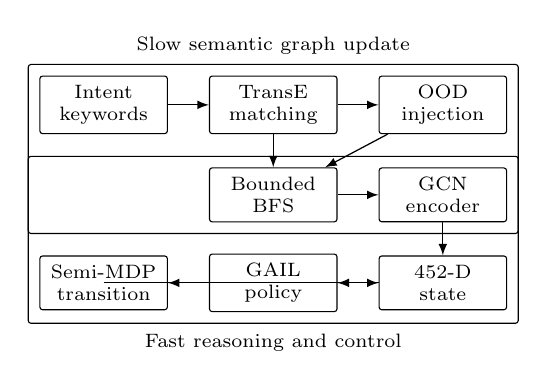
\begin{tikzpicture}[
    node distance=0.42cm and 0.52cm,
    block/.style={draw, rounded corners=1pt, align=center, font=\scriptsize, minimum height=0.58cm, minimum width=1.62cm},
    big/.style={draw, rounded corners=1pt, align=center, font=\scriptsize, inner sep=4pt},
    arr/.style={->, >=latex, line width=0.45pt}
]
\node[block] (intent) {Intent\\keywords};
\node[block, right=of intent] (match) {TransE\\matching};
\node[block, right=of match] (inject) {OOD\\injection};
\node[block, below=of match] (bfs) {Bounded\\BFS};
\node[block, right=of bfs] (gcn) {GCN\\encoder};
\node[block, below=of gcn] (state) {$452$-D\\state};
\node[block, left=of state] (policy) {GAIL\\policy};
\node[block, left=of policy] (env) {Semi-MDP\\transition};
\draw[arr] (intent) -- (match);
\draw[arr] (match) -- (inject);
\draw[arr] (match) -- (bfs);
\draw[arr] (inject) -- (bfs);
\draw[arr] (bfs) -- (gcn);
\draw[arr] (gcn) -- (state);
\draw[arr] (state) -- (policy);
\draw[arr] (policy) -- (env);
\draw[arr] (env) |- (state);
\node[big, fit=(intent)(match)(inject)(bfs), label={[font=\scriptsize]above:Slow semantic graph update}] {};
\node[big, fit=(gcn)(state)(policy)(env), label={[font=\scriptsize]below:Fast reasoning and control}] {};
\end{tikzpicture}
\caption{Implementation flow of the proposed LLM-free semantic reasoning stack. The slow graph update builds an intent-conditioned subgraph, while the fast loop repeatedly performs GAIL-based reasoning over the fixed state interface.}
\label{fig:flow}
\end{figure}

\section{Algorithms and Complexity}

This section presents the training and communication procedures in a style similar to semantic reasoning algorithms in prior implicit semantic-aware communication studies \cite{xiao2024reasoning,xiao2023imitation,zhang2025heteroknowledge}.

\subsection{Offline Training}

The offline stage trains or loads TransE embeddings, constructs the KG interface, generates expert trajectories over pruned subgraphs, and trains the GAIL interpreter. The source side supplies semantic-distance feedback through the discriminator objective, while the destination-side interpreter learns to generate expert-like semantic paths.

\begin{algorithm}[!t]
\caption{Offline Training of the LLM-Free Semantic Interpreter}
\label{alg:offline}
\begin{algorithmic}[1]
\REQUIRE KG triples $\calE$, intent table $\mathcal{T}$, threshold $\tau$, BFS radius $N$, node cap $N_{\max}$, seeds $\mathcal{M}$
\ENSURE TransE embeddings, GCN encoder, GAIL policy $\pi_\theta$, discriminator $D_\phi$
\STATE Train or load TransE entity and relation embeddings.
\STATE Initialize global KG $\KG$ from benchmark triples.
\FOR{each training intent query $q$}
    \STATE Extract entity set $\calC(q)$ from $\mathcal{T}$.
    \FOR{each entity keyword $e\in\calC(q)$}
        \STATE Compute $\mathbf{u}(e)$ and similarity scores to KG entities.
        \IF{$\max_v \cos(\mathbf{u}(e),\mathbf{z}_v)\geq \tau$}
            \STATE Add matched entity $v^\star(e)$ to seed set $\calS_0$.
        \ELSE
            \STATE Inject OOD node $v_e$ and connect it to $\calN_K(e)$.
            \STATE Add $v_e$ to seed set $\calS_0$.
        \ENDIF
    \ENDFOR
    \STATE Extract $\SG_N(q)$ by multi-source BFS with $|\calV_N|\leq N_{\max}$.
    \STATE Encode $\SG_N(q)$ with GCN to obtain $\mathbf{g}_{\SG}$.
    \STATE Generate expert path samples using BFS-based semantic oracle.
    \STATE Roll out $\pi_\theta$ in the Semi-MDP to collect policy samples.
    \STATE Update $D_\phi$ using \eqref{eq:gail_d}.
    \STATE Update $\pi_\theta$ using \eqref{eq:gail_reward} and \eqref{eq:policy_loss}.
\ENDFOR
\RETURN trained interpreter $(\pi_\theta,D_\phi)$ and encoder parameters.
\end{algorithmic}
\end{algorithm}

Algorithm~\ref{alg:offline} is intentionally modular. If a stronger KG embedding model or a human-provided expert path set is available, it can replace the corresponding step without changing the state dimension. Likewise, the source comparator can be upgraded from the discriminator reward to a more explicit semantic-distance metric.

\subsection{Online Communication}

During online communication, the slow loop is triggered when a new query arrives or the intent changes. The resulting subgraph is reused for multiple fast decisions. This is the main source of latency reduction.

\begin{algorithm}[!t]
\caption{Online Intent-Conditioned Semantic Communication}
\label{alg:online}
\begin{algorithmic}[1]
\REQUIRE Query $q$, global KG $\KG$, trained encoder, policy $\pi_\theta$, channel state sampler
\ENSURE Recovered semantic path $\hat{u}_v$
\STATE Extract intent entities $\calC(q)$ and intent vector $\mathbf{i}$.
\STATE Match or inject each entity to form seed set $\calS_0$.
\STATE Build $\SG_N(q)$ with bounded multi-source BFS.
\STATE Compute subgraph embedding $\mathbf{g}_{\SG}$.
\STATE Initialize current node $v_0$ from $\calS_0$ and path $\hat{u}_v\leftarrow \emptyset$.
\FOR{$t=0,\ldots,H_{\max}-1$}
    \STATE Sample or estimate CSI vector $\mathbf{c}_t$.
    \STATE Construct state $\mathbf{s}_t=[\mathbf{z}_{v_t};\mathbf{g}_{\SG};\mathbf{i};\mathbf{c}_t]$.
    \STATE Select semantic action $a_t\sim\pi_\theta(\cdot|\mathbf{s}_t)$.
    \STATE Map $a_t$ to a neighbor/relation decision in $\SG_N(q)$.
    \STATE Append selected relation and entity to $\hat{u}_v$.
    \IF{target semantic condition is satisfied}
        \STATE \textbf{break}
    \ENDIF
\ENDFOR
\RETURN $\hat{u}_v$.
\end{algorithmic}
\end{algorithm}

\subsection{Complexity}

Let $|\calV|$ and $|\calE|$ denote the size of the working KG, $d_e=128$ the entity embedding dimension, $N_{\max}=64$ the subgraph node cap, and $E_N$ the number of edges in the pruned subgraph. A naive full scan for TransE matching costs $O(|\calV|d_e)$ per keyword. This can be reduced by approximate nearest-neighbor indexing, but the prototype keeps the full scan for transparency. OOD injection adds $O(|\calV|d_e+K)$ time for top-$K$ semantic neighbors. Bounded BFS costs $O(N_{\max}+E_N)$ after seeds are selected. GCN encoding costs approximately $O(E_Nd_h+N_{\max}d_hd_o)$ for hidden dimension $d_h$ and output dimension $d_o$. The fast policy forward pass costs $O(d_s h+h^2L+h|\calA|)$ for state dimension $d_s=452$, width $h=512$, and hidden depth $L=3$.

The important distinction is between one-time slow-loop cost and repeated fast-loop cost. If one semantic subgraph is used for $H$ fast decisions, the amortized per-decision latency is
\begin{equation}
\bar{T}(H)=\frac{T_{\mathrm{match}}+T_{\mathrm{BFS}}+T_{\mathrm{GCN}}}{H}
+T_{\mathrm{policy}}+T_{\mathrm{env}}.
\label{eq:amortized_latency}
\end{equation}
This expression explains why a system that appears expensive at the moment of intent switching can still be efficient for continuous control.

\begin{table}[!t]
\centering
\caption{Computational cost of major modules.}
\label{tab:complexity}
\begin{tabular}{lcc}
\toprule
Module & Cost driver & Typical role\\
\midrule
Intent lookup & $O(|q|)$ & local keyword extraction\\
TransE matching & $O(|\calV|d_e)$ & semantic seed selection\\
OOD injection & $O(|\calV|d_e+K)$ & cold-start anchoring\\
Bounded BFS & $O(N_{\max}+E_N)$ & subgraph extraction\\
GCN encoding & $O(E_Nd_h)$ & graph compression\\
Policy forward & $O(d_sh+h^2L)$ & fast semantic action\\
Discriminator & $O((d_s+d_a)h+h^2L)$ & imitation reward\\
\bottomrule
\end{tabular}
\end{table}

\section{Analytical Properties}

\subsection{Pruning Radius from TransE Decay}

Let $\Psi(d)$ be the expected TransE semantic similarity between an intent seed and nodes at graph distance $d$:
\begin{equation}
\Psi(d)=
\bbE\left[
\cos(\mathbf{z}_{v_0},\mathbf{z}_{v})
\;|\;\operatorname{dist}(v_0,v)=d
\right].
\label{eq:psi}
\end{equation}
The measured decay $\Psi(d)$ gives a practical way to choose BFS radius. If the semantic marginal gain beyond depth $N$ is smaller than the marginal cost, deeper expansion is not useful. Let
\begin{equation}
\Delta\Psi(N)=\Psi(N)-\Psi(N+1)
\end{equation}
and let $\Delta C(N)$ be the additional extraction and encoding cost. A radius criterion is
\begin{equation}
N^\star =
\min\left\{N:
\Delta\Psi(N)\leq \lambda_C \Delta C(N)
\right\}.
\label{eq:nstar}
\end{equation}
The repository therefore includes both $\Psi(d)$ measurement and $N\in\{1,2,3\}$ scan scripts.

\subsection{OOD Injection Stability}

Consider the GCN encoder in \eqref{eq:gcn_embedding}. Suppose one OOD node is inserted, perturbing the normalized adjacency and feature matrix by $\Delta\tilde{A}$ and $\Delta X$. If $\sigma$ is 1-Lipschitz and $\|W_\ell\|_2\leq L_\ell$, then the first-order perturbation satisfies
\begin{multline}
\|\Delta \mathbf{g}_{\SG}\|_2
\leq
L_0L_1\left(
\|\Delta\tilde{A}\|_2\|X\|_F
+\|\tilde{A}\|_2\|\Delta X\|_F
\right)\\
+O(\|\Delta\tilde{A}\|_2^2).
\label{eq:ood_bound}
\end{multline}
Because the injected node connects only to $K$ semantic neighbors and the subgraph is capped at $N_{\max}$ nodes, both perturbation terms are bounded. This does not prove that injection always improves semantic fidelity, but it shows why nearest-neighbor injection should not destabilize the GCN representation under controlled $K$ and $N_{\max}$.

\subsection{Policy Jump Under Intent Switching}

Let two consecutive intents produce subgraph embeddings $\mathbf{g}$ and $\mathbf{g}'$. If the spectral-normalized policy has Lipschitz constant $L_\pi$, then for states sharing the same current-node and CSI components,
\begin{equation}
\|\pi_\theta(\cdot|s)-\pi_\theta(\cdot|s')\|_{\mathrm{TV}}
\leq L_\pi \|s-s'\|_2
=L_\pi \|\mathbf{g}-\mathbf{g}'\|_2.
\label{eq:tv_bound}
\end{equation}
If the two subgraphs overlap by
\begin{equation}
\alpha=\frac{|\calV_N\cap\calV_N'|}{|\calV_N\cup\calV_N'|},
\end{equation}
a coarse mean-pooling bound gives
\begin{equation}
\|\mathbf{g}-\mathbf{g}'\|_2
\leq \kappa(1-\alpha),
\end{equation}
and therefore
\begin{equation}
\|\pi_\theta-\pi_\theta'\|_{\mathrm{TV}}
\leq L_\pi\kappa(1-\alpha).
\label{eq:overlap_bound}
\end{equation}
This result explains two design choices: keeping subgraphs local around intent seeds and applying spectral normalization in the generator \cite{miyato2018spectral}.

\subsection{Semantic-Fidelity and Latency Tradeoff}

Let $F(N)$ be expected semantic fidelity with BFS radius $N$, and let $T(N)$ be the slow-loop latency. Trading fidelity against transmission cost is also central to adjustable-rate semantic transmission \cite{li2023fast,gunduz2025jscc}. The useful operating point solves
\begin{equation}
\max_N F(N)-\lambda T(N), \quad N\in\{1,2,\ldots,N_{\max}^{\mathrm{hop}}\}.
\end{equation}
If $F(N)$ is increasing and concave while $T(N)$ is increasing and convex, then the optimal radius is the smallest $N$ for which
\begin{equation}
F(N+1)-F(N)\leq \lambda [T(N+1)-T(N)].
\end{equation}
The empirical $\Psi(d)$ decay acts as a proxy for $F(N+1)-F(N)$. This is why semantic similarity decay and latency profiling should be reported together.

\section{Prototype Evaluation}

\subsection{Datasets and Experimental Settings}

The project targets three KG benchmarks. FB15K237 contains 14,541 entities, 237 relations, about 272K training triples, and about 20K test triples. WN18RR contains 40,943 entities, 11 relations, and about 87K training triples. NELL-995 contains 75,492 entities, 200 relations, and about 150K training triples. The current implementation contains scripts for full TransE training, $\Psi(d)$ measurement, $N^\star$ scanning, end-to-end comparison, convergence evaluation, latency decomposition, OOD robustness, BFS/GCN profiling, and Lipschitz profiling.

The available checkpoint reports FB15K237 TransE evaluation over 20,466 test triples with MRR 0.2806, Hits@1 0.1915, Hits@3 0.3143, and Hits@10 0.4564. These values are used to document the current prototype state rather than to claim state-of-the-art KG completion.

\begin{table}[!t]
\centering
\caption{Benchmark setup and current TransE checkpoint.}
\label{tab:datasets}
\begin{tabular}{lccc}
\toprule
Dataset & Entities & Relations & Training triples\\
\midrule
FB15K237 & 14,541 & 237 & 272K\\
WN18RR & 40,943 & 11 & 87K\\
NELL-995 & 75,492 & 200 & 150K\\
\midrule
FB15K237 MRR & \multicolumn{3}{c}{0.2806}\\
FB15K237 Hits@1 & \multicolumn{3}{c}{0.1915}\\
FB15K237 Hits@3 & \multicolumn{3}{c}{0.3143}\\
FB15K237 Hits@10 & \multicolumn{3}{c}{0.4564}\\
\bottomrule
\end{tabular}
\end{table}

\subsection{Baselines}

The prototype includes three principal comparison modes. The first is the proposed dynamic-pruned method, which extracts an intent-conditioned subgraph with OOD injection. The second is a static hierarchy-like baseline that mimics a fixed semantic layer, in the spirit of hierarchy-aware multi-stage implicit semantic reasoning \cite{sun2026hierarchy}. The third is a no-pruning baseline that exposes the policy to a much larger subgraph, representing an iRML-style setting without dynamic pruning \cite{xiao2024reasoning,xiao2023imitation}. These baselines are not intended as definitive comparisons against all published systems; rather, they isolate the value of dynamic pruning and bounded state construction inside the same code base.

\subsection{Latency Decomposition}

Table~\ref{tab:latency} summarizes the local latency trace. A pure online semantic loop is represented by a 1.2 s per-query baseline. The fast-slow loop executes fast decisions in a few milliseconds. The amortized setting assumes one slow-loop update per 200 fast decisions.

\begin{table}[!t]
\centering
\caption{Prototype latency decomposition from local traces.}
\label{tab:latency}
\begin{tabular}{lccc}
\toprule
Architecture & Mean (ms) & P99 (ms) & Speedup\\
\midrule
Pure online semantic loop & 1201.883 & 1701.934 & 1.0$\times$\\
Fast-slow loop & 2.441 & 3.680 & 492.3$\times$\\
Fast-slow amortized & 8.438 & 11.019 & 142.4$\times$\\
\bottomrule
\end{tabular}
\end{table}

\begin{figure}[!t]
\centering
\includegraphics[width=\linewidth]{../experiments/figures/fig2_latency.pdf}
\caption{Latency trace generated by the project experiment scripts. The result illustrates the benefit of amortizing semantic graph updates across fast control decisions.}
\label{fig:latency}
\end{figure}

The most important observation is not merely the average speedup; it is the change in where computation occurs. In the pure online setting, semantic interpretation is in the critical path at every query. In the proposed fast-slow architecture, expensive graph operations are moved to intent-switching events, and repeated decisions reuse the resulting subgraph embedding. This matches the operation of many wireless control applications, where an intent such as ``avoid collision'' or ``monitor substation'' persists for multiple decision steps.

\subsection{TransE Semantic Decay and Radius Selection}

The measured TransE semantic decay is shown in Table~\ref{tab:psi}. The similarity drops sharply from distance 0 to distance 1 and continues to decrease through distance 3. The decay becomes small near distance 4. This supports scanning small BFS radii rather than expanding deeply into the KG.

\begin{table}[!t]
\centering
\caption{Measured TransE semantic similarity decay $\Psi(d)$.}
\label{tab:psi}
\begin{tabular}{lccc}
\toprule
Distance $d$ & $\Psi(d)$ & Avg. nodes & Decay from $d=0$\\
\midrule
0 & 1.0000 & 299.0 & 0.00\%\\
1 & 0.4932 & 2719.0 & 50.68\%\\
2 & 0.3653 & 8424.8 & 63.47\%\\
3 & 0.3004 & 1277.4 & 69.96\%\\
4 & 0.2973 & 128.6 & 70.27\%\\
5 & 0.3484 & 23.6 & 65.16\%\\
6 & 0.3456 & 10.6 & 65.44\%\\
\bottomrule
\end{tabular}
\end{table}

The non-monotone tail at distances 5 and 6 reflects sparse frontier sampling rather than a reliable semantic recovery. In a final large-scale experiment, this measurement should be repeated for each dataset and seed. For the present prototype, it justifies using $N\in\{1,2,3\}$ as the main scan range.

\subsection{Convergence Behavior}

Fig.~\ref{fig:conv} shows the prototype multi-seed convergence trace. Dynamic pruning produces compact 64-node subgraphs and allows the GAIL policy to train in a controlled local state space. The no-pruning baseline uses much larger subgraphs and has weaker early progress in the smoke-test traces.

\begin{figure}[!t]
\centering
\includegraphics[width=\linewidth]{../experiments/figures/fig1_convergence.pdf}
\caption{Prototype convergence trace comparing dynamic pruning and baseline behavior. The figure documents the current training pipeline and should be regenerated with the full planned seed and epoch budget for final claims.}
\label{fig:conv}
\end{figure}

Convergence in this setting should be interpreted carefully. The reward is sparse because the policy must reach a semantic target through a graph path. A poor subgraph can make the target unreachable regardless of policy quality. Therefore, convergence reflects both reasoning policy learning and slow-loop semantic selection. This coupling is exactly why the paper reports pruning, OOD injection, and policy learning together.

\subsection{OOD Robustness}

Fig.~\ref{fig:ood} shows the prototype OOD robustness and threshold-ablation trace. The purpose of OOD injection is not to guarantee that every unknown term becomes useful; it is to prevent unknown entities from being silently discarded. In low-SNR and sparse-graph settings, injection can improve reachability by anchoring the unknown term near semantically similar known entities. In other settings, it may introduce noisy edges if the nearest neighbors are poor. This motivates reporting injection on/off and threshold sweeps.

\begin{figure}[!t]
\centering
\includegraphics[width=\linewidth]{../experiments/figures/fig3_ood_robustness.pdf}
\caption{Prototype OOD robustness and threshold ablation. Dynamic injection preserves a graph location for unknown intent terms and enables the destination policy to reason through newly added semantic nodes.}
\label{fig:ood}
\end{figure}

\begin{table}[!t]
\centering
\caption{OOD robustness summary from smoke-test traces.}
\label{tab:ood}
\begin{tabular}{lccc}
\toprule
SNR and setting & Mean reward & Fidelity & Goal rate\\
\midrule
$-5$ dB, injection off & -0.3000 & 0.0000 & 0.0000\\
$-5$ dB, injection on & 0.5500 & 0.0833 & 0.0833\\
0 dB, injection off & -0.3000 & 0.0000 & 0.0000\\
0 dB, injection on & -0.3000 & 0.0000 & 0.0000\\
5 dB, injection off & -0.3000 & 0.0000 & 0.0000\\
5 dB, injection on & 0.5542 & 0.0833 & 0.0833\\
10 dB, injection off & 2.2458 & 0.2500 & 0.2500\\
10 dB, injection on & 0.5375 & 0.0833 & 0.0833\\
\bottomrule
\end{tabular}
\end{table}

Table~\ref{tab:ood} shows why OOD injection must be treated as a design parameter rather than a universal improvement. At some SNRs, injection improves recovery from zero; at 10 dB in the smoke-test run, the non-injection setting obtains a higher reward. This can occur when the OOD term is not needed for the sampled target or when injected edges distract the BFS oracle. A publication-grade experiment should therefore include confidence intervals, more episodes per configuration, and threshold-specific analysis.

\subsection{BFS and GCN Profiling}

The BFS/GCN latency profile shows that the first GCN call can include initialization overhead, while subsequent calls are dominated by BFS extraction for 64-node subgraphs. Typical GCN encoding after warm-up is about 1--3 ms in the local trace, whereas BFS extraction varies with graph neighborhood structure. This indicates that optimizing neighbor indexing and seed matching may provide more benefit than replacing the small GCN.

\begin{table}[!t]
\centering
\caption{Representative BFS/GCN latency samples for 64-node subgraphs.}
\label{tab:bfs_gcn}
\begin{tabular}{lccc}
\toprule
Query & Edges & BFS (ms) & GCN (ms)\\
\midrule
0 & 75 & 45.44 & 273.21\\
1 & 78 & 70.87 & 1.87\\
2 & 75 & 59.26 & 1.51\\
3 & 119 & 26.26 & 2.32\\
4 & 119 & 26.46 & 1.92\\
5 & 78 & 67.81 & 1.98\\
\bottomrule
\end{tabular}
\end{table}

The first row includes cold-start overhead and should not be interpreted as steady-state GCN latency. The remaining rows support the fast-slow decomposition: graph extraction is a slow-loop operation, while policy decisions after encoding can be fast.

\subsection{Ablation Axes}

Table~\ref{tab:ablations} summarizes the ablations supported by the implementation. These are important because a semantic communication system can appear to work for the wrong reason. For example, a policy may perform well because the subgraph is tiny and the target is easy, not because it learned robust reasoning. Conversely, a no-pruning baseline may fail because of search-space size rather than an inherently inferior semantic model.

\begin{table}[!t]
\centering
\caption{Implemented ablation axes and diagnostic questions.}
\label{tab:ablations}
\footnotesize
\begin{tabular}{p{0.30\linewidth}p{0.60\linewidth}}
\toprule
Ablation & Diagnostic question\\
\midrule
$N\in\{1,2,3\}$ scan & Does semantic gain saturate before BFS latency grows?\\
Injection on/off & Does OOD anchoring improve reachability under unknown entities?\\
Dynamic vs. static pruning & Does intent-conditioned pruning adapt better than fixed hierarchy?\\
No pruning & How costly is exposing the policy to a large KG region?\\
Spectral norm on/off & Does policy smoothness improve after intent switches?\\
SNR sweep & Does reasoning remain reliable under degraded CSI?\\
Threshold sweep & How sensitive is matching to the OOD decision boundary?\\
\bottomrule
\end{tabular}
\end{table}

\subsection{Comparison With Reasoning-Based Implicit SemCom}

The proposed framework is aligned with reasoning-based implicit semantic communication in its use of explicit semantics, hidden paths, and imitation-style path generation. Its distinctive contribution is to make the semantic front end local, deterministic, and bounded. Table~\ref{tab:comparison} summarizes the conceptual comparison.

\begin{table}[!t]
\centering
\caption{Conceptual comparison with reasoning-based implicit semantic communication.}
\label{tab:comparison}
\footnotesize
\begin{tabular}{p{0.32\linewidth}p{0.27\linewidth}p{0.29\linewidth}}
\toprule
Aspect & Reasoning-based implicit SemCom & This paper\\
\midrule
Semantic substrate & Source/destination knowledge bases & Dynamic KG subgraph\\
Explicit semantics & Detected entities/relations & Keyword entities\\
Implicit semantics & Reasoning paths & KG paths in pruned subgraph\\
Learning method & G-RML-style imitation & GAIL over Semi-MDP\\
Front-end model & General semantic detector possible & LLM-free deterministic extractor\\
Fast-loop state & Method-dependent & Fixed 452-dimensional contract\\
OOD handling & Not the central focus & Dynamic KG injection\\
\bottomrule
\end{tabular}
\end{table}

This comparison is not a claim that the proposed deterministic extractor is more expressive. It is less expressive by design. The point is to provide a reproducible lower-complexity baseline and to show how much semantic reasoning can be obtained from KG structure, imitation learning, and controlled graph pruning alone.

\section{Protocol Operation and Synchronization}

The preceding sections describe the learning architecture. This section specifies how the components operate as a communication protocol. The additional details are useful because semantic communication systems can otherwise blur the boundary between what is learned offline, what is transmitted online, and what is assumed to be shared by the users.

\subsection{Semantic Packet Format}

The source does not transmit the full pruned subgraph in every fast-loop step. Instead, it transmits a compact semantic packet whenever the intent changes or the source detects that the receiver's semantic state is stale. A minimal packet can be written as
\begin{equation}
\mathsf{p}=
\left[
\mathsf{id}(q),\;
\mathsf{seed}(\calS_0),\;
\mathsf{hash}(\SG_N),\;
\mathsf{cfg},\;
\mathsf{crc}
\right],
\label{eq:packet}
\end{equation}
where $\mathsf{id}(q)$ is an intent identifier, $\mathsf{seed}(\calS_0)$ encodes the matched or injected seed nodes, $\mathsf{hash}(\SG_N)$ identifies the subgraph version, $\mathsf{cfg}$ stores pruning parameters such as $N$, $N_{\max}$, $\tau$, and $K$, and $\mathsf{crc}$ is a consistency check. The destination reconstructs or verifies the same subgraph using its local KG and the common KG. If the hash does not match, the destination can request a subgraph refresh or fall back to a smaller seed-only reasoning mode.

This packet format separates semantic identity from channel coding. The channel may carry $\mathsf{p}$ as bits, semantic symbols, or a JSCC latent representation. The present paper focuses on the semantic layer; therefore, the packet abstraction is sufficient for analyzing whether the destination receives enough structured information to run the interpreter.

\subsection{Subgraph Versioning}

Dynamic OOD injection creates a synchronization issue: a source-side injected node must correspond to the same semantic object at the destination. We assign each injected entity a tuple
\begin{equation}
\mathsf{ood}(e)=
\left[
\mathsf{name}(e),\;
\operatorname{TopK}_{v\in\calV}\cos(\mathbf{u}(e),\mathbf{z}_v),\;
\mathsf{time},\;
\mathsf{scope}
\right].
\end{equation}
The top-$K$ neighbor list acts as a semantic fingerprint. If both users share the common KG and embedding model, they can independently verify whether the injected node is anchored to the same region. The scope field controls persistence. A session-scoped OOD node is used only for the current communication episode; a persistent OOD node is stored for future tasks after validation.

Subgraph versioning is important for avoiding silent semantic drift. Suppose the source injects ``micro-drone'' near drone, camera, and surveillance, while the destination injects it near toy, device, and hobby. The resulting reasoning paths may diverge even if the same string is used. A hash over the ordered seed list, neighbor anchors, relation labels, and pruning configuration provides a lightweight consistency test.

\subsection{Semantic Acknowledgement}

Traditional acknowledgements confirm packet reception. A semantic acknowledgement should confirm that the destination has recovered the intended meaning with sufficient confidence. Let $\hat{u}_v$ be the destination path and let $u_E$ be an expert or source-side reference path. A semantic acknowledgement can report a scalar score
\begin{equation}
\mathsf{ack}_{\mathrm{sem}}=
\one\left\{
d_{\mathrm{sem}}(\hat{u}_v,u_E)\leq \epsilon_{\mathrm{sem}}
\right\},
\end{equation}
where $d_{\mathrm{sem}}$ is a semantic distance. In the GAIL prototype, the discriminator reward can serve as a learned proxy for this distance. A more explicit implementation could combine path overlap, TransE endpoint similarity, and relation-type agreement:
\begin{multline}
d_{\mathrm{sem}}(\hat{u},u)
=
\lambda_e\left[1-\cos(\mathbf{z}_{\hat{v}_L},\mathbf{z}_{v_L})\right]\\
+\lambda_r d_R(\hat{r}_{1:L},r_{1:L})
+\lambda_p d_P(\hat{u},u),
\end{multline}
where $d_R$ compares relation sequences and $d_P$ compares path structure. This mirrors the semantic-distance role of source-side comparators in reasoning-based implicit semantic communication, while remaining compatible with the KG implementation \cite{xiao2024reasoning,wheeler2025causal,peng2026simac}.

\subsection{Failure Handling}

Four failure modes are especially relevant.
First, no intent keyword may be matched. The fallback entity set $\{\mathrm{general},\mathrm{communication}\}$ prevents a null state, but it should trigger low-confidence reporting. Second, a keyword may be matched to an unrelated KG node because the embedding space is weak. This is mitigated by the threshold $\tau$ and by OOD injection. Third, the target semantic node may be absent from the pruned subgraph. This is mitigated by scanning $N$ and by reporting reachability statistics. Fourth, the channel may corrupt the semantic packet. This is handled by the packet hash and by retransmitting only the compact semantic configuration rather than the whole KG.

\begin{table}[!t]
\centering
\caption{Protocol fields and their functions.}
\label{tab:packet}
\begin{tabular}{l p{0.63\linewidth}}
\toprule
Field & Function\\
\midrule
Intent ID & Identifies the current communication task or service objective.\\
Seed list & Specifies matched and injected KG entities used by BFS.\\
Subgraph hash & Verifies source-destination consistency after pruning.\\
Configuration & Stores $N$, $N_{\max}$, $\tau$, $K$, and encoder version.\\
Semantic ACK & Reports whether the destination meaning is sufficiently close.\\
\bottomrule
\end{tabular}
\end{table}

\subsection{Interaction With Radio Resource Control}

The current action space is represented as a 128-way categorical decision. In a more complete wireless stack, this action can be factorized following intent- and resource-aware semantic networking \cite{qin2025genai,krayani2026aav}:
\begin{equation}
a_t=(a_t^{\mathrm{sem}},a_t^{\mathrm{bw}},a_t^{\mathrm{mcs}},a_t^{\mathrm{rep}}),
\end{equation}
where $a_t^{\mathrm{sem}}$ chooses the next KG relation or neighbor, $a_t^{\mathrm{bw}}$ chooses bandwidth, $a_t^{\mathrm{mcs}}$ chooses modulation and coding, and $a_t^{\mathrm{rep}}$ chooses repetition or retransmission level. The fixed state contract remains useful because semantic decisions and radio decisions share the same input features. Under poor CSI, the policy may prefer shorter semantic packets, more robust coding, or paths that rely on already synchronized KG context. Under strong CSI, the policy can transmit richer seed information or update OOD anchors more aggressively \cite{yang2025swinjscc,devoto2026token,li2023fast}.

\section{Conclusion}

This paper presented an LLM-free implicit semantic-aware communication framework based on intent-conditioned KG pruning and imitation reasoning. The source side maps intent keywords to KG seeds, injects OOD entities when necessary, and extracts a bounded BFS subgraph. The destination side encodes the subgraph with a GCN and uses a GAIL policy to generate implicit semantic paths over a Semi-MDP. The fixed 452-dimensional state contract decouples slow semantic graph updates from fast control decisions. Analytical results explain the pruning-radius tradeoff, OOD injection stability, and policy sensitivity under intent switching. Prototype traces demonstrate substantial latency reduction and validate the evaluation pipeline, while also showing that final TWC-grade claims require rerunning the planned multi-seed experiments. The framework offers a reproducible baseline for KG-based semantic communication in settings where LLM/LAM dependence is undesirable.

\bibliographystyle{IEEEtran}
\bibliography{refs}

\end{document}
